\documentclass[a4paper,man,floatsintext,natbib]{apa6}

\usepackage[english]{babel}
\usepackage[utf8x]{inputenc}
\usepackage{amsmath}
\usepackage{graphicx}
\usepackage[colorinlistoftodos]{todonotes}
\usepackage{nameref}
\usepackage{upquote}
\usepackage{listings}


\title{A Reproducible MEEG Data Analysis Workflow with conda, Snakemake, and R~Markdown}
\shorttitle{Reproducible MEEG Workflow}
\author{Evgenii Kalenkovich, Egor Levchenko}
\affiliation{HSE University}

\abstract{This tutorial is devoted to computational reproducibility, which is an ability to recreate the reported results using the original data and code. Previous studies show that this is impossible for a large percentage of studies with published data and code. We find this situation to be a serious problem for science in general and for the cognitive neuroscience in particular. In this tutorial, we focused on three sources of irreproducibility: differences in software environment, utilization of out-of-date derivative files, and human errors during manual copying of figures, tables, and numbers to the manuscript. We describe three tools that solve these issues: conda, Snakemake, and R Markdown, respectively. Together, they form an effective toolkit that can help researchers achieve reproducibility of their analyses. We demonstrate an application of this toolkit by reimplementing a published data analysis pipeline applied to an open MEEG dataset. Main strengths and weaknesses of our and other approaches are discussed.}


\begin{document}
\maketitle

\section{Introduction}
In this tutorial, we describe an approach to performing of MEEG analyses that are computationally reproducible, i.e. identical results can be obtained by running the same code on the same data.
We describe different aspects of trying to achieve this goal:
(a) creating and maintaining reproducible computational environments with software versions as close as possible to those used originally,
(b) using workflow management systems that help ensure that all the derivative files are continuously up-to-date and do so efficiently,
(c) using literate programming so that all numbers and plots in the manuscript are derived directly from the data and not copy-pasted manually.
Combining all three of these aspects ensures computational reproducibility of your results and makes it possible for your future self, for your colleagues and for other researchers to reproduce your results once the data and code are published.

Here, we define \emph{reproducibility} (more precisely, \emph{computational reproducibility}) as an ability to obtain exactly the same results that were reported in the publication, using the same data and code that were used by the original authors. 
This is in contrast to \emph{replicability}: obtaining similar experimental results (in terms of hypothesis test results and effect sizes) by using the same experimental design and analysis but applying it to new data.
The necessity of replicability is taken for granted by some \citep{pashlerReplicabilityCrisisOverblown2012a,opensciencecollaborationEstimatingReproducibilityPsychological2015} and considered more skeptically by others \citep{devezerCaseFormalMethodology2021}.
However, we find it hard to imagine anyone arguing that computational reproducibility is not essential for good scientific practice. The whole replicability question is moot if it is not possible to reproduce the original results in the first place.

The issue of reproducibility might seem trivial at first: publish your data and your code - and voilà - anyone can reproduce your results. Unfortunately, the reality is far from this naive understanding. Multiple studies \citep{stockemerDataAccessTransparency2018,obelsAnalysisOpenData2020,hardwickeDataAvailabilityReusability2018} showed that, in a large percentage of cases it was impossible to reproduce the reported results, even though the data and the code were available. We are not aware of any empirical studies testing the computational reproducibility of MEEG, so we have to rely on anecdotal evidence and common sense here. The attempts of current study's authors to reproduce several MEEG results have not been successful even once: it usually took considerable time to even make the code run at all - only for it to output results that were vastly different from the ones reported. Also, we believe that everyone has either first-hand or second-hand experience with "I haven't changed anything but the code does not work anymore or produces different results". In this tutorial, we present our approach by applying it to the analysis presented in \cite{jasReproducibleMEGEEG2018a}. In that paper, the authors show how a comprehensive analysis of an MEG dataset reported earlier \citep{wakemanMultisubjectMultimodalHuman2015} can be recreated in a reproducible manner. Despite their explicit effort to make the analysis reproducible and the fact that the code accompanying the paper is well-documented and clearly organized, we were not able to run their code without updating it and rerunning the whole analysis (which takes about a week to complete) several times. Finally, MEEG analysis is usually quite involved and relies on solutions from multiple toolboxes and custom code, so we have no reason to believe that the situation should be any better than in other fields.

We find the following sources of irreproducibility to be the main culprits: changes in the software environment, out-of-date derivative files, and human error during copying the analysis outputs to the manuscript.

More often than not, someone else's, or your own older code will not run at all and throw errors instead. The reason is that exactly the same code will not run in a computationally different environment. As the software is updated, its API changes and, for example, the same function calls can require a different number of parameters, optional parameters can become mandatory, etc. You can update the code to reflect these changes but it is likely that the output of the function will change as well. With the software updates also comes the dependence on new pieces of software or on other versions of the previously existing dependencies. So, updating the code is often insufficient. 
Often, despite the fact that the versions of the main pieces of software were reported in the manuscript, it is still impossible to reproduce the environment.
Sometimes the description is insufficient because seemingly minor but important pieces of software were not reported.
Other times, separate pieces might have incompatible dependencies.
Finally, reproducing the environment could financially prohibiting in the case when you have a different version of commercial software (MatLab, SPSS, etc.).

The first part of the solution is to rely on open-source, free scientific software as much as possible, so that anyone can have access not only to the software itself but also to the specific version that you used. Once you do this, you can use an environment management system to manage all your software dependencies, including dealing with their complicated inter-dependencies and keeping track of all the versions. In this tutorial, we will use a tool named \emph{conda} for that.

In practice, reproducibility comes in two distinct flavors: the \emph{final-product} reproducibility of an already finished analysis and the \emph{ongoing} reproducibility of an analysis as it evolves from a script that gathers the experimental data all the way to the publishable manuscript. The final-product reproducibility can, in theory, be checked by running a single master script. With MEEG, it can take a while, but if you are lucky enough and the results do not change, you will only need to run it once at the time, as you are not changing the analysis anymore, anyway.
Realistically, however, you will not be running your analysis just once when the analysis pipeline is completed, but rather run it incrementally, at different stages of the analysis development. 
Here, however, the master script approach breaks: it is impractical to wait for the whole analysis to be rerun when you need to continue working on the other steps.
There are ad-hoc solutions to this problem involving commenting out pieces of code, adding code to compare file modification times, adding custom configuration files, etc.
But these solutions are extremely error-prone.
Instead, we recommend delegating dealing with these issues to a workflow management system.
Such tools help you run only the specific bits of the analysis that were affected by any changes you might have made.
In this tutorial, we will use a tool named \emph{Snakemake} for that.
In addition, it will automatically make your analysis execution more efficient through automatic parallelization.

The final important source of irreproducibility is the manual copying of numbers and figures from the analysis software to the text editing software. We recommend using literate programming approaches, in which the text is interspersed with bits of code that produce all the numbers and the plots that go into the final rendered document. This eliminates the possibility of making a manual copying error, by eliminating the copying step altogether: all data-derived outputs in the manuscript are directly connected to the underlying data. In this tutorial, we will use a tool named \emph{R~Markdown} for that.

In sum, we will show how to make your MEEG analysis reproducible, using \emph{conda} to make the software environment reproducible, \emph{Snakemake} to make and keep the analysis outputs up to date, and \emph{R~Markdown} to keep the manuscript connected to the underlying data. The usage of conda and R~Markdown is the same, whether you are working with MEEG or other types of data, so we will be brief and refer you to other sources of information where necessary. With Snakemake, we will go into much more detail because this tool was developed and is mainly used in the bioinformatics context, which does not translate easily to MEEG. After describing the tools, we will walk you through applying them to the analysis reported in \cite{jasReproducibleMEGEEG2018a} (which, itself, is a reanalysis of the \cite{wakemanMultisubjectMultimodalHuman2015} dataset).

\section{Tools}
In this section, we describe the tools that help us tackle the three causes of irreproducibility: (a) conda will help avoid differences in the software environment, (b) Snakemake will help keep all the derivative files up-to-date and do so efficiently, and (c) R Markdown will help to remove the disconnect between the numbers and figures in the manuscript and the underlying data. 
Out of these three, only Snakemake requires consideration specific to MEEG analysis.
Therefore, for Snakemake, we provide a comparably detailed guide while we describe conda and R~Markdown rather briefly.
At the end, we mention several other helpful tools: git, BIDS, renv, and Docker.

\subsection{Software Environment Management}
\label{section:conda}
In order for your code to produce the same results upon later execution, it is necessary that it is run using exactly the same versions of as many pieces of software as possible. A practical and user-friendly solution to this problem is to use the software package management system, \emph{conda}, and the so-called \emph{conda environments} it allows one to manage. Conda is probably most widely known as that part of the Anaconda data science distribution that lets you install Python packages. However, conda is not just a Python package manager, rather it is a software package management system or, citing the conda documentation: "Package, dependency and environment management for any language - Python, R, Ruby, Lua, Scala, Java, JavaScript, C/ C++, FORTRAN, and more"\footnote{https://docs.conda.io/en/latest/}. As long as you stick to free (not always necessarily open-source) software, conda will cover most of your reproducible software environment needs.

Technically, the conda environment is a directory that contains a number of \emph{conda packages} that you install into this environment. You can \emph{activate} this environment in a terminal, after which the code that you run from that terminal, will use the software from that directory. The power of conda environments comes from the fact that a \emph{conda package} might be a Python package, but it can also be Python itself, R, a number of other languages, a command-line utility, etc. Moreover, all of these will be installed in an isolated environment, in which your code is run against the specific versions of these packages, while not affecting other code run on your system.

Conda can be installed as part of the Anaconda distribution or through its small, bootstrap version \emph{miniconda}. You can check that conda is available on the terminal by running \verb|conda --version| in it. Consult the conda documentation in case of any issues. A new environment called, for example, \verb|reproducible_MEEG|, can be created and activated with

\begin{verbatim}
conda create -n reproducible_MEEG
conda activate reproducible_MEEG
\end{verbatim}

After the environment is activated, \verb|(reproducible_MEEG)| is added at the beginning of the command line. You can install Python of a specific version (3.7 her) with

\begin{verbatim}
conda install python=3.7
\end{verbatim}

To see all the packages installed in the environment, you can run \verb|conda list|. To save a list with all the packages to a file, you can use

\begin{verbatim}
conda env export > environment-full.yml
\end{verbatim}

This command creates a YAML\footnote{"YAML is a human friendly data serialization language for all programming languages" (from https://yaml.org/)}-formatted file called \verb|environment-full.yml| containing the list. Unfortunately, we cannot directly use this file to reproduce the environment later: due to differences in operating systems and hardware architecture, a small proportion of the packages will differ from one computer to another. Some packages, e.g. \verb|vs2015_runtime|, are necessary on Windows but are not needed and actually do not exist for Linux/macOS. So, if you create \verb|environment-full.yml| on Windows, you will not be able to recreate the environment on other systems. As a workaround to this problem, we will use a manually populated file that we will call \verb|environment.yml| (the environment definition files can be named anything but using \verb|environment.yml| will signal to other users what this file contains). In this file, we will keep track of the packages that we specifically install, but not their dependencies. This approach leads to less reproducible environments in the sense that some packages might differ in their versions. In another sense, however, they are more reproducible because it will be more likely that an environment can be recreated on a different computer, albeit with some differences. In practice, these differences are usually inconsequential (because the main packages \emph{are} tracked). For cases where they are not, we recommend keeping the conda-populated \verb|environment-full.yml| as well. This allows one to pin down possible execution differences to specific packages. Following is an example of a minimal \verb|environment.yml| file:

\begin{verbatim}
dependencies:
  - python=3.7
\end{verbatim}

When conda installs a package, it downloads it from the Anaconda package repository. This repository is divided into subsections called \emph{channels}. Unless configured otherwise, \verb|conda install| looks for packages in the channel called \emph{defaults}. A large number of scientific software packages is located in the \emph{conda-forge} channel; the workflow management system, \emph{Snakemake}, that we will later use, is in the \emph{bioconda} channel. To install a package from a specific channel, use \verb|conda install -c <channel_name> <package_name>=<version>|. For example, \emph{mne 0.23.0}, from the \emph{conda-forge} channel, can be installed with

\begin{verbatim}
conda install -c conda-forge mne=0.23.0
\end{verbatim}

As you install more packages into an environment, installing a new package might lead to the change in the version of an earlier installed package, rendering \verb|environment.yml| invalid. To avoid this situation and catch the package dependency conflicts early, we recommend to avoid using \verb|conda install| altogether and instead update the environment based on the \verb|environment.yml| file. To add a package from a specific channel, use \verb|<channel_name>::<package_name>=<version>|. For example, adding \emph{mne 0.23.0} from the \emph{conda-forge} channel and \emph{snakemake-minimal 6.2.1} from the channel \emph{bioconda} (we use the minimal version of Snakemake here because - unlike the full version - it is available for Windows as well) will look as follows:

\begin{verbatim}
dependencies:
  - python=3.7
  - bioconda::snakemake-minimal=6.2.1
  - conda-forge::mne=0.23.0
\end{verbatim}

To update the environment after introducing changes to \verb|environment.yml|, use

\begin{verbatim}
conda env update -n reproducible_MEEG -f environment.yml --prune
\end{verbatim}

Flag \verb|-n| signals the environment name, \verb|-f| - the name of the environment definition file. The last flag, \verb|--prune|, instructs conda to remove packages that are no longer needed. It does not change anything in this case but it is useful when you remove a package or change some packages' versions. It is a good practice to use this flag with any update and let conda figure out whether it was necessary.

Tracking the packages you add in \verb|environment.yml| is the bare minimum requirement for the environment reproducibility and it is a good idea to track more. There is no simple rule to decide which packages to track. Some rules of thumb include tracking packages that you directly use in your code and tracking widely used packages, such as \emph{pandas}, \emph{scipy}, \emph{matplotlib}, \emph{numpy}, etc. Another reason to add additional packages to \verb|environment.yml| is the hidden incompatibilities of some packages with newer versions of some of their dependencies. For example, \emph{snakemake-minimal 6.2.1} is incompatible with new versions of its dependency, \emph{smart\_open}. This can be remedied by downgrading it to version 3 by adding \verb|conda-forge::smart_open=3| to \verb|environment.yml| and updating the environment.

Some Python packages are not available directly through conda but only through the Python Package Index (\emph{PyPI}) and installed using the \emph{pip} package manager. In this case, add pip itself to \verb|environment.yml| and any PyPI packages under a separate pip node:

\begin{verbatim}
dependencies:
    ...
  - pip=21.0.1
  - pip:
    - pybids=0.13.2
\end{verbatim}

Finally, if you use R, install it through conda as well: multiple versions are available in the conda-forge channel. It is possible to install and track R packages directly through conda but this approach might be limiting. Instead, we recommend using a dedicated R package manager, \emph{renv}.

Summing up using conda environments:

\begin{enumerate}
    \item Use a separate environment for each project.
    \item Add new packages to \verb|environment.yml| without specifying the version unless you need a specific version.
    \item Create or update the environment file with \verb|conda env update -n <environment-name> -f environment.yml --prune|
    \item After each change, update the full environment specification with \verb|conda env export > environment-full.yml| and pin the newly installed package versions in \verb|environment.yml|.
    \item Add additional packages to \verb|environment.yml| to increase reproducibility, consulting \verb|environment-full.yml| for their version.
\end{enumerate}

\subsection{Snakemake}
\label{section:snakemake}
Let us start with an oversimplified illustrative example. Suppose we have electroencephalography (EEG) data from 20 subjects, recorded during an oddball task and all we want to do is compare P300 between the standard and the deviant conditions with a paired t-test. For each subject, we have a single recording file, \verb|data/subXX_raw.fif|, where XX is the subject code going from 01 to 20. We will run our analysis in three steps, assuming that we already have the code that does each one of them:

\begin{enumerate}
    \item Clean and epoch each \verb|data/subXX_raw.fif| file and save the results to \verb|epoched/subXX_data.fif| (done by function \verb|clean_and_epoch(path_to_raw, path_to_epoched)|).
    \item Using each \verb|epoched/subXX_data.fif|, calculate P300 in both conditions and save to \verb|P300/subXX_P300.csv| (done by function \verb|calculate_P300(path_to_epoched, path_to_P300)|).
    \item Using all of the \verb|P300/subXX_P300.csv| files, create a pdf report, \verb|manuscript.pdf|, with the results of the test and a plot of P300 values (done by function \verb|make_report(path_to_P300_list, path_to_manuscript|).
\end{enumerate}

This analysis pipeline is schematically drawn in Figure~\ref{fig1} below.

\begin{figure}
\centering
\captionsetup{justification=centering}
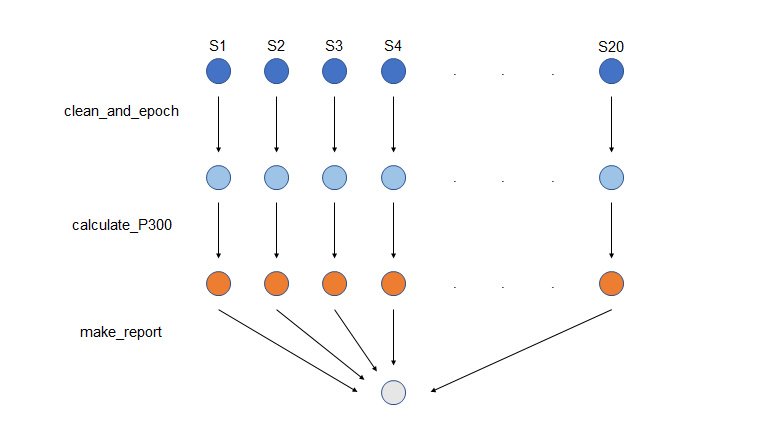
\includegraphics[width=\textwidth]{pictures/Figure1_pipeline.png}
\caption{Each node in the graph represents a file and arrows are Python function calls. First bunch of files (first line of blue nodes) are raw files for subjects from 1 to 20, the second bunch of files (light blue) is a result of applying the $clean\_and\_epoch$ function, the third bunch is obtained after calculating P300 properties (orange), and the final file is a manuscript (light gray).} \label{fig1}
\end{figure}

Often, such an analysis would be managed through a \emph{master script} that might look like this:

\begin{verbatim}
for subject in subjects:
    clean_and_epoch(path_to_raw=..., path_to_epoched=...)
for subject in subjects:
    calculate_P300(path_to_epoched=..., path_to_P300=...)

make_report(path_to_P300_list=[... for subject in subjects],
            path_to_manuscript='manuscript.pdf')
\end{verbatim}

(In the code above, the ellipses stand for the string-manipulation code, for assembling the appropriate path strings for a given subject code.) In our oversimplified example, the master script is very short and simple, but in a real-life scenario it quickly gets large and unwieldy. It still, however, does the job, if you want to rerun the whole analysis assuming there are no errors and no missing files. There are a couple of problems with this approach though.

First of all, it is inefficient: a lot of the function calls could be done in parallel. This is true, both for individual calls of, for example, \verb|clean_and_epoch|, but also for calls of \verb|calculate_P300|, once most of the \verb|clean_and_epoch| calls are finished and there are idle processors.

Second, a lot of times there \emph{are} errors \emph{and} missing files. Considering that a lot of MEEG processing steps take considerable time, it is impractical to rerun the whole analysis when an error is fixed or a missing file is provided, which only affects a part of the pipeline. The same is true for when a piece of code is updated. So, in practice, the researcher will either not use the master script at all, after a fix or a change, because it would take too long to run, or they would comment out some of the lines and tweak the script in other ways, so that it only runs what is necessary. Both options are very error-prone and are very likely to lead to derivative files that are out of date and non-reproducible outputs.

Third, the pipeline usually quickly becomes too large to hold in one's head and requires visualization to describe and analyse. With the master script approach, this usually requires hand-made drawing of all the interwoven dependencies in the pipeline. These are hard to keep up-to-date with the master script and check for consistency.

Of course, all the issues described above could be solved by adding pipeline managing code of varying difficulty to the master script: parallelization code is relatively straight-forward, managing file state and visualizing the inter-dependencies of individual steps would be more involved. That would be an unnecessary waste of the researcher's time and effort spent on coding. Or, they could be solved by the researcher being extra careful. Which would be very error-prone while also being  an unnecessary waste of the researcher's time and effort spent on \emph{executing} the code. A more reliable and simpler solution is to outsource these efforts to a \emph{workflow management system}. In this tutorial, we will show an example of such a system called \emph{Snakemake} (for those familiar with \emph{make}, Snakemake is \emph{make} with the added flexibility brought by allowing Python code in the Makefiles).

Snakemake is most prevalently used in bioinformatics \citep{molderSustainableDataAnalysis2021a}. It shares some features with MEEG research: large files, complicated analysis pipelines, combination of multiple tools in the same analysis, parallelizable independent steps. This makes Snakemake a good fit for our purposes. With Snakemake, you define the analysis pipeline in terms of \emph{rules} for each of the steps that transform a number (one or more) of existing files into a number (one or more) of new ones. Snakemake then takes care of running the pipeline with parallelization, without rerunning unnecessary steps, with monitoring outdated files and it can visualize the pipeline in the form of a directed acyclic graph (DAG).

The pipeline description is written to a file usually called simply "Snakefile" (no extension). This file contains a set of rules to create each of the derived files in the pipeline. Most often a rule consists of four parts: its name, the \emph{output} - the file(s) that this rule helps to create, the \emph{input} - the file(s) that are required to create the output, and the instructions on how to generate the output from the input. The instructions can come in different forms (more on that later), for this example we will assume that it is a piece of Python code. A basic rule has the following form (note the colons and the indents):

\begin{verbatim}
rule <rule_name>:
    input:
        <input_file>
    output:
        <output_file>
    run:
        <python_code>
\end{verbatim}
For example, a rule to create \verb|epoched/sub01_epo.fif| might look like this:

\begin{verbatim}
rule clean_and_epoch_subject_01:
    input:
        'data/sub01_raw.fif'
    output:
        'epoched/sub01_epo.fif'
    run:
        clean_and_epoch(input[0], output[0])
\end{verbatim}

Note that the Python code in the \verb|run| section does not use explicit paths to the input/output files but instead refers to the via Python lists \verb|input| and \verb|output|. We will soon see that this not only helps us avoid repeating ourselves but also makes rules flexible. The reason we have to add \verb|[0]| after \verb|input| and \verb|output| is that generally there can be multiple input and output file paths and thus \verb|input| and \verb|output| refer to the lists of the paths even when they contain a single element.

To create \verb|epoched/sub01_epo.fif|, we can ask Snakemake to make it for us with

\begin{verbatim}
snakemake epoched/sub01_epo.fif --cores 1
\end{verbatim}

In this case, the file to be created is referred to as the \emph{target file}. Here, we assumed that the code is run in the same directory where the \verb|Snakefile| is located and that it is actually called \verb|Snakefile|. In this case, there is no need to specify the location explicitly. In other cases, use \verb|-f <path_to_Snakefile>| command-line argument. The argument \verb|--cores 1| tells Snakemake to use a single processing core. Throughout this section, we will assume there is only one core; adjust this parameter in case you want to use more cores.

Another way to create \verb|epoched/sub01_epo.fif| is to tell Snakemake to run the rule \verb|clean_and_epoch_subject_01|:

\begin{verbatim}
snakemake clean_and_epoch_subject_01 --cores 1
\end{verbatim}

In this case, the rule to be run is referred to as the \emph{target rule}. Finally, you could simply run 

\begin{verbatim}
Snakemake --cores 1
\end{verbatim}

Without additional specifications, Snakemake will use the first rule it finds in the Snakefile as the target rule.

Note that the rule \verb|clean_and_epoch_subject_01| could theoretically be used on any subject if the subject number could be allowed to vary. Snakemake makes this possible via the use of \emph{wildcards}, which are named variable parts of the input/output paths. Using a wildcard, we can define a single rule that is able to create any of the epoched files (note that the wildcard name \verb|subject_number| is put inside curly brackets):

\begin{verbatim}
rule clean_and_epoch:
    input:
        'data/sub{subject_number}_raw.fif'
    output:
        'epoched/sub{subject_number}_epo.fif'
    run:
        clean_and_epoch(input[0], output[0])
\end{verbatim}

We can then ask Snakemake to create any of the epoched files. For example, after the following command:

\begin{verbatim}
snakemake epoched/sub06_epo.fif
\end{verbatim}

Snakemake would

\begin{enumerate}
    \item Look for rules whose output matches \verb|epoched/sub06_epo.fif| for some value of the wildcard
    \item Determine that \verb|clean_and_epoch| is the only such rule.
    \item Determine that the value of the wildcard \verb|subject_number| is \verb|06|.
    \item Plug this wildcard into the input resulting being \verb|data/sub06_raw.fif|.
    \item Check that the input exists.
    \item Run the code in the \verb|run| section of the rule.
\end{enumerate}

Note that step 2 would fail if we deleted \verb|epoched/sub01_epo.fif| and asked Snakemake to recreate it because there would be two rules that could create this file. See Snakemake documentation for solutions to this problem should it arise in your own pipeline. Here, we will simply virtually delete \verb|clean_and_epoch_subject_01| to avoid this collision.

Unlike with the rule \verb|clean_and_epoch_subject_01|, it does not make sense to ask Snakemake to just run the rule \verb|clean_and_epoch| because while the rule can create any of the \verb|*_epo.fif| files, it does not specify any specific ones that it would output. This applies to any rule with wildcards in the output: Snakemake needs to know which files to create so these rules cannot be used as target rules. Instead, it is customary to have a dummy rule \verb|all| as the first rule in the file and have any output files in the current state of the pipeline as its inputs:
\begin{verbatim}
rule all:
    input:
        [f'epoched/sub{subject_number}_epo.fif'
         for subject_number in subject_numbers]
\end{verbatim}

Where \verb|subject_numbers| is the list of character strings: \verb|'01'|, \verb|'02'|, \verb|...|, \verb|'20'|. Plugging a number of possible wildcard values is a common action when working with Snakemake, so it has a special function that simplifies the process - \verb|expand|. Instead of the list comprehension above, one could simply write

\begin{verbatim}
rule all:
    input:
        expand('epoched/sub{subject_number}_epo.fif',
               subject_number=subject_numbers)
\end{verbatim}

In case of multiple wildcards, you can add them as another keyword argument to \verb|expand| - in that case Snakemake will use all the possible combinations of the elements of the supplied lists. Sometimes, what you want instead is to plug the wildcards in a row-wise fashion: plug the first element from each of the wildcard lists, then the second, etc. This can be achieved by supplying \verb|expand| with the second positional argument \verb|zip| (this can be any function that creates combinations of elements from multiple lists, \verb|zip| is the one to achieve row-wise selection). Finally, sometimes you want to plug in some wildcards but not the others. In this case, supply only those you want to plug as keyword arguments and add \verb|allow_missing=True| at the end.

If you run command \verb|snakemake| in the console, it will:

\begin{enumerate}
    \item Find the target rule - the first rule in the Snakefile which is the rule \verb|all|.
    \item Determine which files are missing from its input. 
    \item Determine that the rule \verb|clean_and_epoch| is capable of producing each of these files.
    \item For each of the necessary files, prepare a separate independent invocation of \verb|clean_and_epoch| which is referred to as a \emph{job}.
    \item Run all the \verb|clean_and_epoch|-based jobs in an arbitrary order.
    \item Run an \verb|all|-based job (as this is a dummy rule does not really do anything, neither will this job).
\end{enumerate}

Before running Snakemake, it is advisable to check how many jobs will be run from each rule, and check whether the numbers match your expectations without running the jobs themselves, in what is referred to as \emph{dry run}. To do so, add \verb|--dry-run| flag to the Snakemake call, or \verb|-n| for a shorter version.

The dummy \verb|all|-based job can only be run once all the \verb|clean_and_epoch|-based jobs are done - when its input files are all created. The \verb|clean_and_epoch|-based jobs, however, can be run independently and thus can be parallelized. Snakemake does this automatically if you tell it to use more processing cores with the \verb|--cores <n>| argument.

The rest of the pipeline can be defined with the following rules:

\begin{verbatim}
rule all:
    input:
        'manuscript.pdf'
rule clean_and_epoch:
    input:
        'data/sub{subject_number}_raw.fif'
    output:
        'epoched/sub{subject_number}_epo.fif'
    run:
        clean_and_epoch(input[0], output[0])
rule calculate_P300:
    input:
        'epoched/sub{subject_number}_epo.fif'
    output:
        'P300/sub{subject_number}_P300.csv'
    run:
        calculate_P300(input[0], output[0])
rule make_report:
    input:
        expand('P300/sub{subject_number}_P300.csv',
               subject_number=subject_numbers)   
    output:
        'manuscript.pdf'
    run:
        make_report(input, output[0])
\end{verbatim}

There are several things to note about this version of Snakefile. First, the rule \verb|all| includes only the \verb|manuscript.pdf| file but not the epoched files or the P300 csv files. The reason for this is that the latter files become redundant once we have the whole pipeline defined. When \verb|manuscript.pdf| is the target file, Snakemake will have to run \verb|make_report| to create it. To do that, it will need all the P300 csv files, to create each of which it will need to run a \verb|calculate_P300| job, which will require the corresponding epoched files. To create each of those, it will need to run a \verb|clean_and_epoch| job, which will require the corresponding raw files. Thus, the only file we need to explicitly ask Snakemake for is \verb|manuscript.pdf|. Second, note that \verb|make_report| does not have any wildcards in the output specification and thus can be run directly as the target rule without the need to run the dummy \verb|all| rule. It is advisable to nevertheless keep rule \verb|all|. Finally, in the \verb|run| section of the rule \verb|make_report| we use \verb|input| instead of \verb|input[0]| because we need to supply the whole list of input files to the \verb|make_report| function.

There are a few ways that Snakefile can be cleaned a bit in order to avoid repetition and increase clarity. We will create variables containing the wildcard templates for the file paths instead of repeating them in every rule. We will name the input and outputs so that we can refer to them in the \verb|run| section with \verb|input.<name>| instead of \verb|input[0]|. We will refer to the outputs of previous rules instead of defining the paths directly. For this, we can use a variable \verb|rules| that allows us to refer to the field of any rule defined above. For example, output of the rule \verb|clean_and_epoch| can be referred to as \verb|rules.clean_and_epoch.output| in any of the rules defined below that rule. Here is what a cleaner Snakefile might look like:

\begin{verbatim}
raw_template = 'data/sub{subject_number}_raw.fif'
epoched_template = 'epoched/sub{subject_number}_epo.fif'
p300_template = 'P300/sub{subject_number}_P300.csv'
manuscript_filename = 'manuscript.pdf'
rule all:
    input:
        pdf = manuscript_filename 
rule clean_and_epoch:
    input:
        raw = raw_template
    output:
        epoched = epoched_template
    run:
        clean_and_epoch(input.raw, output.epoched)
rule calculate_P300:
    input:
        epoched = rules.clean_and_epoch.output.epoched
    output:
        p300 = p300_template 
    run:
        calculate_P300(input[0], output[0])
rule make_report:
    input:
        p300_list = expand(rules.calculate_P300.output.p300,
                           subject_number=subject_numbers)   
    output:
        pdf = manuscript_filename
    run:
        make_report(input.p300_list, output.pdf)
\end{verbatim}

With a pipeline this small, it is not hard to hold it whole in the working memory. As pipelines get larger, however, it is easier to visualize all the dependencies in the pipeline using a graph similar to those depicted in Figure~\ref{fig1}. Snakemake provides ways to create such images both at the rule level (as in Figure~\ref{fig2}) and at the job level (as in Figure~\ref{fig3}). To do so, first install the \verb|graphviz| utility (also available as a conda package in the \verb|conda-forge| channel). To create a rule-level graph, use

\begin{verbatim}
snakemake --rulegraph | dot -Tpng > rulegraph.png
\end{verbatim}

And for the job-level graph, use

\begin{verbatim}
snakemake --dag | dot -Tpng > jobgraph.png
\end{verbatim}

\begin{figure}
\centering
\captionsetup{justification=centering}
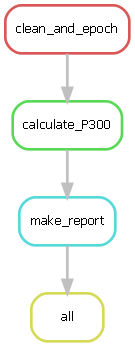
\includegraphics[height=3in,width=3in,keepaspectratio]{pictures/Snakemake_rulegraph.png}
\caption{Rules graph of P300 example.} \label{fig2}
\end{figure}

\begin{figure}
\centering
\captionsetup{justification=centering}
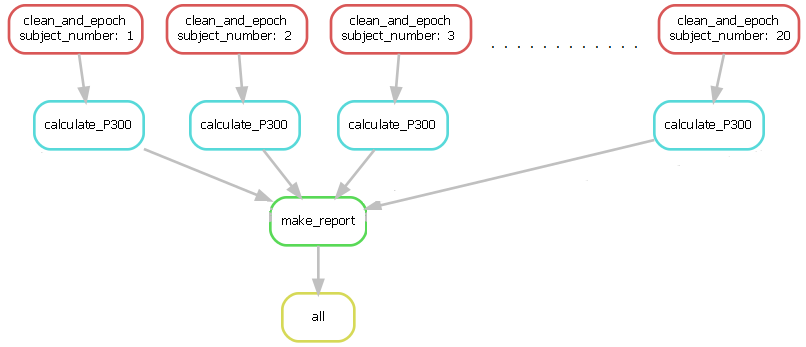
\includegraphics[height=\textheight,width=\textwidth,keepaspectratio]{pictures/Snakemake_dag_graph_cut.png}
\caption{Graph of jobs of P300 example.} \label{fig3}
\end{figure}

Both the \verb|--rulegraph| and \verb|--dag| flags tell Snakemake to produce text-based graphs in the graph description language DOT. The \verb|dot| utility from Graphviz then translates it into visual form. The \verb|-Tpng| flag tells \verb|dot| to save the output in a png graphics format. Consult the Graphviz documentation for other output formats. The \verb|rulegraph.png| and \verb|jobgraph.png| names are arbitrary, you can use anything else.

Let us assume that the way we calculate the P300 has to be changed (for example, it was calculated using the wrong set of sensors). After making the appropriate changes to the \verb|calculate_P300| function, all we need to do is run Snakemake again telling it that the \verb|calculate_P300| rule has to be rerun using the \verb|--forcerun| flag (or, shorter - \verb|-R|) flag:

\begin{verbatim}
snakemake --forcerun calculate_P300
\end{verbatim}

This will result in the recalculation of all the \verb|*_P300.csv| files and recreation of \verb|manuscript.pdf|. Importantly, the rule \verb|clean_and_epoch| will not be run at all because our change to the code of the \verb|calculate_P300| function does not influence this earlier step in the pipeline. So, how does Snakemake understand that the rule \verb|make_report| has to be rerun but the rule \verb|clean_and_epoch| - does not? In this specific case, we told Snakemake explicitly to rerun the \verb|calculate_P300| rule, so it can assume that its outputs - the  \verb|*_P300.csv| files - will be updated. Thus, the input of the \verb|make_report| rule will have changed which will \emph{trigger} its rerun. This is similar to the thought process underlying a manual execution of a pipeline like this: the researcher figures out what lines in the master script must be rerun because of the change in the code, then comments out the lines that came before and reruns the master script. In this particular case, the manual solution is simple enough. However, as the processing pipeline becomes more involved and especially when it becomes non-linear, the manual solution becomes increasingly complicated and, more importantly, highly error-prone. Snakemake takes care of tracking the inter-dependence of individual steps and figures out which of them have to be rerun automatically.

Upon changing the code of the function  \verb|calculate_P300|, you might want to test the corresponding rule without triggering the \emph{downstream} rules - rules that depend on the outputs of  \verb|calculate_P300| either directly or through a sequence of rules. To do so, one might create a temporary rule whose input includes all the  \verb|*_P300.csv| files. Another way is to tell Snakemake to start running the whole pipeline but stop after all the jobs \emph{spawned} by the  \verb|calculate_P300| rule are finished using the \verb|--until| flag:

\begin{verbatim}
snakemake --forcerun calculate_P300 --until calculate_P300
\end{verbatim}

Once you have checked that the code and the corresponding rule work as expected, you can run Snakemake without any additional flags and Snakemake will run all the rules that have to be rerun but not any other rules. In this case, Snakemake is not told explicitly that the rule \verb|calculate_P300| was updated so it will rely on the more general prinicple: any rule that the target rule depends on will be rerun if the modification date of any of its inputs is later that the modification date of some of its outputs. In our case, Snakemake will see that the target rule \verb|all| depends on the rule \verb|make_report| whose inputs (the updated \verb|*_P300.csv| files) were modified after its output (\verb|manuscript.pdf|) was. Therefore, Snakemake will rerun the rules \verb|make_report| and \verb|all|. The rule \verb|make_report| depends on the rule \verb|calculate_P300| which, in turn, depends on the rule \verb|clean_and_epoch|. However, both of these rules have outputs that were updated after their inputs, so Snakemake will not rerun them. 

The same logic of comparing the modification times applies when only some of the files of the same type have been updated. Let us assume, for example, that one of the files with raw data was mislabelled: \verb|data/sub02_raw.fif| is actually a copy of \verb|data/sub01_raw.fif| and so you substitute the correct file for it. Again, you can account for this in a master script: you will have to restrict all the subject-level codes to subject "02", leave the group-level code as is and rerun the script. This, however, is even more error-prone than the case above. Snakemake will take care of it for you automatically: you just need to set the modification date of the new correct \verb|data/sub02_raw.fif| to the current time so that it is newer than any of the derivative files and rerun Snakemake without any additional flags. It will then spawn a single job from each of the subject-level rules (\verb|clean_and_epoch| and \verb|calculate_P300|) and rerun the group-level rules (\verb|make_report| and \verb|all|).

Using Snakemake also helps when there is an execution error in one of the jobs.
Suppose that the mislabelled file \verb|data/sub02_raw.fif| did not just have the wrong data but was also the wrong kind of file altogether. Most probably, in this case, the function \verb|clean_and_epoch| will throw an error and halt. By default, when a single job spawned by a rule does not finish successfully, Snakemake will halt the overall execution and delete all the outputs of that rule and any of the downstream rules that might have finished. However, sometimes, including the current example, this is undesirable: the subject-level rules \verb|clean_and_epoch| and \verb|calculate_P300| can be run on all the other subjects. To tell Snakemake to run as many jobs as it can when it stumbles upon an error, add a flag \verb|--keep-going|.

Up to this point, we have only been using Python for the actual processing. When you do so, you can put any Python code under the "run" node of a rule. However, as long as your code can be run from the command line, you can use Snakemake to run it. In this case, the command should be put as a string in the \verb|shell| node. For example, if the \verb|clean_and_epoch| function was implemented in Matlab and saved to a \verb|clean_and_epoch.m| file, we could use it as follows:

\begin{verbatim}
rule clean_and_epoch:
    ...
    shell:
        "matlab -r 'clean_and_epoch({input.raw}, {output.epoched})'"
\end{verbatim}

Note that because we used the \verb|shell| node, the command is quoted, because for Snakemake it is a Python string, and the inputs and outputs are referred to using the curly brackets. There is also an execution node \verb|script| which allows one to use a Python, R, Julia, or Rust script (Matlab is not supported) or an R~Markdown document (it will be rendered according to the first output option in the yaml front matter). In all these scripts, there will be a special object \verb|snakemake| in the environment that will allow the script to access the input and output file paths of the corresponding rule. See Snakemake documentation for more details.

In conclusion, Snakemake allows one to define the processing pipeline independently from the implementation of individual steps and execute that pipeline with automatic parallelization all while ensuring that all the derivative files are continuously up-to-date. Using Snakemake improves the replicability of your project directly - by allowing you to keep the pipeline updated efficiently with only the necessary computational steps rerun, and indirectly - by offloading the task of tracking the file dependencies from the researcher to their computer and thus minimizing the chance of error.

\subsection{Literate Programming}
Multiple reproducibility problems stem from simple mistakes made during copying analysis outputs (numbers, figures) from the analysis software to the text editing software. Tracking what has or has not been updated in the manuscript manually is extremely error-prone. A solution to this problem is using literate programming: interleaving the text with pieces of code that produce all the data-driven outputs. These pieces are executed during the process called \emph{rendering} resulting in the final product that contains all the numbers and figures directly derived from your data.

There are multiple implementations for literate programming, the one we recommend is called \emph{R~Markdown}. It is run using the R software environment but is capable of executing code in Python, SQL, and multiple other languages. The code pieces can either come between text paragraphs in which case they are called \emph{chunks} or directly inside the paragraphs where they are called \emph{inline code}. A code chunk is put between lines \verb|```{r}```| and \verb|```|, a piece of inline code - between \verb|`r| and \verb|`| (\verb|r| tells R~Markdown that you want to execute this code using R). At the very beginning of an R~Markdown document, there is a section called \emph{YAML front matter} with \verb|---| delineating its beginning and end. The front matter contains the document|s meta information, e.g. the title, and rendering options, e.g. the output format. After the front matter, comes the body, which consists of text formatted using the Markdown language and possibly inline code and the code chunks.

Below is a minimal example of an R~Markdown document. We will assume that the data is in a file called \verb|data.csv| and that there is an R file \verb|functions.r| that contains three functions: \verb|load_data|, \verb|report_t_test|, and \verb|plot_data| with the latter two requiring only the output of the first one to function. The functions are loaded in the line \verb|source("functions.r")|.

\begin{verbatim}
---
title: Reproducible MEEG
output: pdf_document
---
```{r}
source("functions.r")
data <- load_data("data.csv")
```
The test showed the following results: `r report_t_test(data)`.
The raw data are depicted below:
```{r}
plot_data(data)
```
\end{verbatim}

To render the document, you will need R and pandoc installed (use conda packages \emph{r-base} and \emph{pandoc}). After installing R, install the R package \emph{rmarkdown}: run R in the console by printing \verb|r|, then run \verb|install.packages('rmarkdown')| (select any CRAN (R packages repository) mirror if prompted). To render the document, save it to a file, then run inside R:

\begin{verbatim}
rmarkdown::render('<filename.rmd>', envir = new.env())
\end{verbatim}

The latter argument ensures that the code in the document is run in a new R environment thus letting you avoid potential problems when your R session changes certain options, variables, functions, etc. 

In case there is an error during rendering saying that a LaTeX distribution is missing on your machine, you will need to install a \emph{LaTeX} (a typesetting system) distribution as well. The simplest way to obtain one is to install the R package \verb|tinytex| (run \verb|install.packages('tinytex')|) and then run \verb|tinytex::install_tinytex()|. To quit R after the rendering is done, run \verb|quit(save='no')|.

There are multiple packages that extend the capabilities of R~Markdown. One of them is the package called \verb|papaja| that allows you to render R~Markdown to a pdf or a MS Word document formatted according to the APA style guide. The result can then be submitted to the journal as is. Install \verb|papaja| with

\begin{verbatim}
install.packages('remotes')
remotes::install_github('crsh/papaja')
\end{verbatim}

On Windows, you might have to install two additional tools: git and RTools. Read the error messages (if any) for the instructions. Once the installation is complete, run

\begin{verbatim}
rmarkdown::draft("reproducible-MEEG_papaja.rmd", "apa6", 
                 package = "papaja", create_dir = FALSE, edit = FALSE)
\end{verbatim}

This will create an R~Markdown document called \verb|reproducible-MEEG_papaja.rmd| that can be rendered into an APA-compliant document. Go through this document and update the fields in the YAML front matter to reflect your own information. Once you are done, render it with

\begin{verbatim}
rmarkdown::render('reproducible-MEEG_papaja.rmd')
\end{verbatim}

Both editing and rendering R~Markdown documents is facilitated by using an integrated development environment (IDE) for R called RStudio. This is not necessary, however: you can always edit the \verb|.rmd| file in any plain-text editor and render it from the terminal. In fact, we recommend using the console even if you use RStudio to avoid RStudio settings influencing the rendering. Or, better yet, wrap the console code in a Snakemake rule so that the number and the figures are not only derived directly from the analysis outputs, but those outputs themselves are kept up-to-date with your analysis code and raw data. For more information about R~Markdown, read "R~Markdown: The Definitive Guide" by \cite{xieMarkdownDefinitiveGuide2019}.

\subsection{Other tools}
Here, we will briefly mention tools that are helpful when you aim for analysis reproducibility but do not directly contribute to it (git, BIDS) and tools that are simply out of scope of the current tutorial (Docker, renv).

\subsubsection{Git}
Git is a system for version controlling your code and any other text files. It can control non-text-based files as well but is less efficient and useful for that. Remember that reproducibility boils down to applying the same code to the same data and getting the same results. The problem is that it is very hard to check whether the code is the same or not and what has changed if anything has. The situation is even worse in a collaborative setting. Git efficiently solves these problems: it shows you what has changed, when any change happened, what the state of your code was when you ran the analysis last time, etc. And it does all this while allowing for relatively easy collaboration. We highly recommend using git for all your code and code-related (e.g., R~Markdown files) needs. While we find git to be a helpful tool for your reproducible analyses, others find it an essential one \citep{peikertReproducibleDataAnalysis2021a}. Many people find git's learning curve to be steep which we believe to be in part due to the insistence on the part of many tutorials on using git from a terminal. We recommend starting with a graphical user interface (\emph{GUI}), such as GitHub Desktop, GitKraken, SourceTree, GitX, and learn the command-line usage in parallel.
This way, you can already use git while still climbing the learning curve.
We recommend to start with a very basic guide by Roger Dudler\footnote{https://rogerdudler.github.io/git-guide/} and then continue with a more comprehensive one by Sam Livingston-Gray\footnote{http://think-like-a-git.net/}.

\subsubsection{BIDS}
BIDS (Brain Imaging Data Structure) is a standard for organizing both raw and derived neuroimaging data. It does not force you to use any specific data storing formats but instead provides a clear unified way to arrange your data within a specific directory structure and write down the necessary metadata so that your data can be understood and subsequently used by anyone. Using BIDS does not necessarily help with reproducing your own analysis but it certainly facilitates checking the reproducibility and reusing the data by other researchers. Other benefits of formatting your dataset according to the BIDS standard include the ease of reading and handling your data with many tools now being aware of the BIDS data structure, the ease of uploading the dataset to a public repository such as openneuro.org, and the hidden benefit of being forced to store the metadata that you do not use now but you or someone else might require later.

For the toy example above, the BIDS-formatted dataset would look like this:

\begin{verbatim}
BIDS_dataset/
|-- dataset_description.json
|-- sub-01/
|  |-- meg/
|  |  |-- sub-01_task-oddball_meg.fif
|-- sub-02/
   | ...
|-- sub-20/
\end{verbatim}

Notice that the only new file is the \verb|dataset_description.json|. Otherwise, this is exactly the same dataset except for the filenames and the folder structure.

\subsubsection{Renv}
Renv is an R package that manages R dependencies of your projects. Like conda environments, renv environments are separate folders that contain all the installed R packages for your project without affecting other projects. Similarly to the \verb|environment-full.yml| file, renv creates a "renv.lock" file that tracks all the installed R packages together with their versions. Unlike conda, however, this file is cross-platform and there is no need for a separate shortened \verb|environment.yml| file. Even though a large number of R packages can be installed through conda, we recommend using renv for R package management because it is more powerful and more convenient to use. It can't however manage versions of R itself so for that we still need conda.

\subsubsection{Docker}
Docker - like conda and renv - allows one to create and manage isolated software environments - \emph{containers} to use the docker term. Conceptually, docker containers are close to conda and renv environments: they allow you to use a separate set of software pieces without affecting other processes on your machine and it allows other people to recreate this set on their own machine. The difference is that docker containers allow for an even deeper level of isolation and for installation of almost arbitrary software (tracking software versions requires the corresponding installation files to be available for download in the future). In a sense, docker simulates a computer within your computer making it similar to virtual machines. There are certain technical differences between docker containers and virtual machines that make docker containers much easier to use and thus making it practical to run your analysis through them. These two properties together: deeper recreation of the software environment and an ability to use them for everyday work make them a perfect solution for the software environment reproducibility. The only reason that we did not include using docker into this tutorial is that many MEEG researchers - especially in the developing countries (based on admittedly anecdotal evidence from Russia) - still use Windows 7 and Windows Server 2012 in which the use of docker, while possible through virtual machines, is impractical for everyday use. This means that they will neither be able to maintain the ongoing reproducibility of their projects nor check or utilize the final-product reproducibility of the docker-based analyses of other researchers. This fact, of course, does not preclude one from using docker as an additional final-product reproducibility layer once the analysis is done. This way, there is an option to reproduce your environment both with the docker that contains conda and with conda alone. We recommend the following guide for setting up conda within a docker container\footnote{https://towardsdatascience.com/conda-pip-and-docker-ftw-d64fe638dc45 }.

\section{Application to an Open MEEG Dataset}
In this part of the tutorial, we go through the steps of applying our approach to the analysis reported in \cite{jasReproducibleMEGEEG2018a} which is a reanalysis of the MEEG part of the "multi-subject, multi-modal human neuroimaging dataset" \citep{wakemanMultisubjectMultimodalHuman2015} publicly available at openfmri.org (legacy version) and openneuro.org (current version). The article by \cite{jasReproducibleMEGEEG2018a} had an aim closely similar to ours: to show a way to run "A reproducible MEG/EEG Group Study" (from the article title). However, they focused on different aspects of the task than we do. They showcased the MNE software package for MEEG analysis, provided a tutorial that goes beyond the usual single-subject data, applied and compared different strategies at various stages of the analysis, and made all the scripts necessary to reproduce their analysis publicly available. 

In addition, they shared their software environment using a conda environment YAML file (what we name \verb|environment-full.yml| in Section \nameref{section:conda}), ran all the individual scripts (such as \verb|05-run_ica.py| for fitting ICA models for each participant's data) using a dependency-tracking utility GNU Make (which was the inspiration for Snakemake), and generated dynamically-populated reports using the reStructuredText format and the documentation building software tool Sphinx. Thus, their code, in theory, deals with all three areas that we focused on in this tutorial: software environment reproducibility, workflow management, and dynamically populated reporting. However, none of the employed tools are taught in the article. Which is where our tutorial comes in: it extends the one by \cite{jasReproducibleMEGEEG2018a} by teaching the researcher the tools to organize their MEEG analysis in a continuously reproducible way. In other words, \cite{jasReproducibleMEGEEG2018a} showed \emph{what} one can do with an MEEG group dataset whereas we will show you \emph{how} to do so reproducibly.

We would like to highlight several differences in which tools we used and how we used them. First, \cite{jasReproducibleMEGEEG2018a} used a conda environment to manage their software environment and shared it in full in the form of the \verb|environment.yml| that contained all the packages in the environment. This approach, while sensible on the surface level, led to us not being able to reproduce the environment due to one package that was installed from a non-standard channel that does not exist anymore and a few packages incompatible with the operating systems we used (Windows 7 and Windows Server 2012). With some guesswork we could have tried to reproduce the environment closely but, on the advice of a colleague of the original authors, we used the current environment file used for the mne-python package when trying to reproduce the analysis as-is. That is why our advice is to use a shorter environment specification in \verb|environment.yml| for environment recreation and the full specification in \verb|environment-full.yml| for potential tracking of environment differences. Second, while \cite{jasReproducibleMEGEEG2018a} used the dependency-tracking utility GNU Make, they did not use it to track the file dependencies in their analysis and thus avoid unnecessary reruns of the analysis steps. Our tool of choice for this is Snakemake which was inspired by GNU Make but took it a step forward by adding automatic parallelization, more flexible wildcard usage and generally allowing for more flexibility by allowing the user to intersperse the rule definitions with Python code. Third, \cite{jasReproducibleMEGEEG2018a} used Sphinx for creating reports whose content stemmed directly from the data. This is a versatile tool that is capable of creating comprehensive interactive reports as can be readily seen on the site accompanying their paper. However, here we chose R~Markdown instead because its output can be directly submitted to the journal and its learning curve is considerably flatter.

We would like to emphasize that our alternative approach is not meant as a critique of the one taken by \cite{jasReproducibleMEGEEG2018a} but instead as a proposal for an improvement with stronger reproducibility and higher efficiency. Their analysis was well-documented making it relatively easy for us to make occasional changes to the code so that the analysis could be run as a whole. However, we do believe that with a little time investment in learning the tools we describe here, one can make both their life and the life of other people trying to reproduce an analysis easier. This is especially true for learning to use a workflow management system such as Snakemake. On the two-core Linux machine we used to run the \cite{jasReproducibleMEGEEG2018a} analysis in its original form (with occasional code changes), the whole run took around a week. So, every time there was an error, we lost a considerable amount of time: either on rerunning the whole part of the analysis or carefully selecting which parts did not have to be rerun all while not running some other parts that did not depend on the step that produced an error. This is precisely where Snakemake steps in, see Section \nameref{section:snakemake} for a more detailed discussion of the matter.

Finally, there are some differences between the analysis of \cite{jasReproducibleMEGEEG2018a} and the one reported here. First, our conda environment is different as described above. Second, instead of the original \cite{wakemanMultisubjectMultimodalHuman2015} dataset, we used an updated version that is organized according to the BIDS standard \citep{gorgolewskiBrainImagingData2016} and contains only 16 out of 19 participants. These, however, were the same 16 participants analyzed in both the original paper and in the \cite{jasReproducibleMEGEEG2018a} reanalysis. Third, using BIDS-formatted data additionally meant that we did not have to extract the stimulus events from the data as this information is now already present in the dataset. Note that in the original dataset the uploaded "raw" data had been cleaned with MaxFilter \citep{tauluPresentationElectromagneticMultichannel2005} while in the updated dataset, the raw data is truly raw and the MaxFiltered data are under the \verb|derivatives/meg_derivatives| folder. Fourth, for the purposes of the source modeling of the MEEG data, \cite{jasReproducibleMEGEEG2018a} performed reconstruction of the brain structure using the FreeSurfer software distribution \citep{fischlFreeSurfer2012}. Our results of the same procedure were slightly different, possibly due to the difference in the FreeSurfer version which was not specified in \cite{jasReproducibleMEGEEG2018a} article. To avoid this problem, we provide a public repository with the results of the reconstruction and suggest that such data should always be published together with the raw data. Fifth, we had a technical problem with the sliding estimator analysis and skipped this step entirely.

\subsection{Setting up}
The first step is setting up the software environment and the folder structure. Create a folder to store the code for the project. In the beginning, we will install and track the minimal set of software: python, snakemake (requires channels conda-forge and bioconda), and mne (requires channel conda-forge). Here is what our \verb|environment.yml| will look like:

\begin{verbatim}
name: reproduction
channels:
  - defaults
  - conda-forge
  - bioconda
dependencies:
  - python
  - bioconda::snakemake-minimal
  # Otherwise, snakemake throws an error (see https://git.io/JRckv)
  - conda-forge::smart_open=3
  - conda-forge::mne
\end{verbatim}

There are two non-obvious lines here. First, we install the \emph{snakemake-minimal} package here because it is available for Windows as well as Linux/MacOS but still provides all the necessary core functionality. Second, we had to pin the version of the conda package \verb|smart_open| because its newer versions are incompatible with the snakemake-minimal version available from conda-forge at the time of writing (6.2.1). Such tweaks are unfortunately an inevitability but they are usually easily made as necessary with the use of \verb|environment-full.yml|.

For your own analysis, create the environment based on the file above, then create its full description in \verb|environment-full.yml| and then pin the package versions in \verb|environment.yml|. To recreate \emph{our} environment, start by pinning the versions in \verb|environment.yml| as follows: Python 3.9.4, snakemake-minimal 6.2.1, and mne 0.2.2.
Next, create a folder where you will store the raw and the derivative data and set an environment variable to its path. This way, the code can refer to this folder without relying on its location relative to the code location. This is especially helpful when multiple researchers use a shared folder for the data but not the code. We will use the environment variable \verb|reproduction_data|.

Next, you have two options for getting the data. First, you can download the whole dataset from openneuro.org to the data folder. Second, you can rely on a rule that downloads the data for you. The downside of the first option is the increased storage requirement, of the second - connection interruptions that might require multiple passes. Note that the two approaches are not mutually exclusive: if you download the dataset manually, the downloading rule will simply not be triggered. If you choose the manual download route, store the data in the \verb|bids| subfolder.

\subsection{Analysis pipeline}
As an overview of the analysis, here are the major steps in the analysis in \cite{jasReproducibleMEGEEG2018a} that we recreate:

\begin{enumerate}
    \item get cleaned stimulus-locked epochs,
    \item calculate evoked response,
    \item do the forward models for source reconstruction,
    \item do source reconstruction using two alternative techniques,
    \item visualize evoked responses and the reconstructed sources.
\end{enumerate}

Before we start implementing the pipeline proper, we will first create an empty Snakefile and start filling it with a few variables that we will certainly use whatever the rules will be. These are the \verb|bids_dir| and \verb|subject_codes| variables that contain the folder that contains the raw data (subfolder \verb|bids| of the folder stored in the environment variable \verb|reproduction_data|) and the participant codes (\verb|"01"|, \verb|"02"|, etc.) respectively.

There is no defined way to start defining the pipeline. If this is an analysis you have already done on a different dataset earlier, then you might be able to define the whole pipeline before any one of the rules is actually implemented. Start with the rule \verb|all| with a single input: \verb|manuscript.pdf| and then back-trace it all the way to the raw files. To create \verb|manuscript.pdf|, you will need a rule \verb|make_manuscript| that will take as its input: (1) an R~Markdown document, (2) the tabulated data for the descriptive and inferential statistics and any figures created within the document, (3) figures that are created outside of the document. For each of the data and figure inputs, there needs to be another rule with its own inputs that will require more rules to be created, and so on and so on. Until you hit the end which is the raw data. Once all the rules and the corresponding file dependencies are set up, you can start implementing the \verb|run| (or \verb|shell|, or \verb|script|) parts of the rules now going forward from the raw files. To avoid errors, just tell Snakemake to stop at the last rule having been implemented using the \verb|--until| flag.

\subsubsection{Cleaning and Epoching}
We believe that the situation described above, where you are able to anticipate all the things that you will need to do with the data before even touching them, is ideal. It is also utopian. More likely, you will know only parts of it, for example, the way you will clean the data. In this case, decide in what form you will need the cleaned data in and start with that. For the \cite{jasReproducibleMEGEEG2018a} analysis, this is a single file for each of the participants that contains the stimulus-locked data. Loosely following the BIDS standard, we will put each such file in the following folder:

\begin{verbatim}
subj_preproc_dir = (bids_dir / 'derivatives'  
                    / 'preprocessing' 
                    / 'sub-{subject_number}'
                    / 'ses-meg' / 'meg')
\end{verbatim}

We refer the reader to the BIDS documentation for the reasons why this path is as rather complicated as it is. It|s only property important here is that this folder is subject-specific, hence we used the \verb|subject_number| wildcard so that the rules we create are applicable to any of the participants. The path to the files themselves will be

\begin{verbatim}
epochs_cleaned_template = (subj_preproc_dir /
    'sub-{subject_number}_ses-meg_task-facerecognition_epoCleaned.fif')
\end{verbatim}

This path does not follow the BIDS standard because of the non-standard \verb|epoCleaned| but it is close enough for our purposes. Again, the only thing important here is that the filename is subject-specific as well and so we used the same \verb|subject_number| wildcard as above. When Snakemake plugs in the wildcard values, the ones with the same name will get the same value. As you can see, the BIDS standard leads to rather long and complicated paths. This is not a problem in practice but to save space, we will use ellipses for large parts of the paths from here on out. See the accompanying code for the full versions. Now we are ready to start defining rules \verb|all| and \verb|clean_epochs|:

\begin{verbatim}
rule all:
    input:
        clean_epochs = expand(epochs_cleaned_template,
                              subject_number=subject_numbers)
rule clean_epochs:
    input:
        ??? = ???
    output:
        clean_epochs = epochs_cleaned_template
    run:
        pass
\end{verbatim}

Now, we need to trace back our analysis from the \verb|epochs_cleaned_template| back to the raw data. We will not go through each rule and will only focus on the ones whose input-output structure is slightly more complicated than what we described in Section \nameref{section:snakemake}. Let us start with finishing the rule \verb|clean_epochs|. As you can see, the cleaning is done in two ways: the linear filtering is applied at an earlier stage and at the \verb|clean_epochs| stage, the already filtered and epoched data (input №1) is additionally filtered by removing ICA components (the results of fitting ICA to the data is input №2) that we earlier selected as artifactual (the list of artifactual components is input №3). For the actual cleaning, we will use a function \lstinline[breaklines]|clean_epochs(ica_path, artifact_components_path, epochs_path, epochs_cleaned_path)| that takes all the input and output paths as arguments, does the cleaning and save the results to a file at the output path. That the rule and the function share a name will not cause errors, whether you use the same names to highlight their connection or use different names to avoid confusion is the matter of taste. For the purposes of this tutorial, the body of this function (and all the other functions for this matter) is irrelevant. Here is what the next iteration (only the new or changed lines of code) of Snakefile might look like:

\begin{verbatim}
epoched_template = ... / 'sub-{subject_number}..._epo.fif')
ica_template = ... / '{subject_number}..._ica.fif')
artifact_components_template = (... /
    'sub-{subject_number}..._artifactComponents.npz')
rule all:
    input:
        clean_epochs = expand(epochs_cleaned_template,
                              subject_number=subject_numbers)
def clean_epochs(ica_path, artifact_components_path, epochs_path,
                 epochs_cleaned_path):
    ...
rule clean_epochs:
    input:
        epochs = epoched_template,
        ica = ica_template,
        artifact_components = artifact_components_template        
    output:
        clean_epochs = epochs_cleaned_template
    run:
        clean_epochs(
            ica_path=input.ica,
            artifact_components_path=input.artifact_components,
            epochs_path=input.epochs,
            epochs_cleaned_path=output.clean_epochs)
\end{verbatim}

Where \verb|epoched_template|, \verb|ica_template|, and \verb|artifact_components_template| are the variables containing the generalized subject-level paths to the epoched data, fitted ICA model, and select artifactual components respectively. We will not list any more templates and function signatures to save space, all of them can be found in the accompanying code. To implement the pipeline further, we will need rules for creating all of the input files of the \verb|clean_epochs| rule, for creating their input files, etc. You can see the graph of these rules in Figure~\ref{fig4}.

\begin{figure}
\centering
\captionsetup{justification=centering}
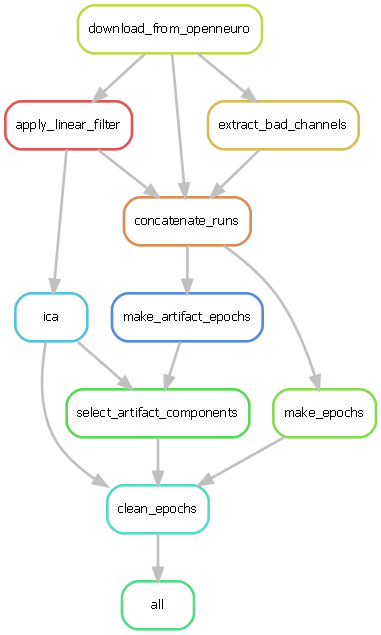
\includegraphics[height=5in,width=5in,keepaspectratio]{pictures/CleanAndEpoch_rulegraph.png}
\caption{The rule graph of the pipeline until clean\_epochs rule.} \label{fig4}
\end{figure}

In our implementation, they all end up depending on the root rule \verb|download_from_openneuro|. This is not necessary, simply skip such a rule if your data are not published yet or you simply want to download them manually. Here, we added this rule mostly to show that rules do not have to have inputs! This rule creates file based on their path relative to \verb|bids_dir| only:
\begin{verbatim}
rule download_from_openneuro:
    output:
        file_path = bids_dir / '{openneuro_filepath}'
    wildcard_constraints:
        openneuro_filepath = openneuro_filepath_regex
    run:
        ...
\end{verbatim}

Another reason for adding this rule is to highlight a common if not very frequent problem: multiple rules are seemingly capable of creating the same files. Here, \verb|download_from_openneuro| seems to be able to download any file in \verb|bids_dir| which is unfortunate because we will put all our derivative files under the same folder. In this case, Snakemake will not be able to determine which rule to use to create some of the files and will throw an error informing you of this ambiguity. One of the possible solutions to this situation is to add so called wildcard constraints - regular expressions that limit what values can a wildcard take. This way, Snakemake will only use \verb|download_from_openneuro| for the files that satisfy these constraints - the ones that we specify to be the source data files for our analysis. Consult Snakemake documentation for more ways to deal with ambiguous rules.

The rules \verb|apply_linear_filter| and \verb|extract_bad_channels| (the latter one extracts the information about the channels marked as bad by the dataset authors) are straightforward with one input and one output file. A more interesting one is rule \verb|ica|. Each participant in the dataset has six MEG recordings - \emph{runs} in the BIDS vernacular. The data from all of them is put together back-to-back before fitting the ICA model. Additionally, before the ICA model is fitted, the data need to be highpassed with 1 Hz being most often used as the lower frequency limit. However, for the rest of the analysis, the data will not be highpassed at all resulting in the files with the filtered data being fully described by three wildcards:

\begin{lstlisting}[breaklines]
filtered_template = (... /
    'sub-{subject_number}_..._run-{run_id}_filteredHighPass{l_freq}.fif')
\end{lstlisting}

The \verb|run_id| can take values from \verb|"01"| to \verb|"06"| and \verb|l_freq| can either be \verb|"1"| or \verb|"None"|. For the input of the \verb|ica| rule, we will need all the participant's runs highpassed at 1 Hz. Importantly, we need to keep the \verb|subject_number| wildcard so that the rule can be used on any participant's data. For that, we will supply only the \verb|run_id| and \verb|l_freq| to the \verb|expand| function (see Section \nameref{section:snakemake}) and tell it to ignore the fact that we skipped \verb|subject_number|:

\begin{verbatim}
rule ica:
    input:
        runs = expand(filtered_template, 
                      run_id=run_ids, l_freq="1",
                      allow_missing=True)
    output:
        ica = ica_template
    run:
        calculate_ica(input.runs, output.ica)
\end{verbatim}

Where \verb|run_ids| is the list of possible run codes: \verb|"01"|, \verb|"02"|, ..., \verb|"06"|. A similar approach is used in the rule \verb|concatenate_runs| that concatenates non-highpass-filtered data for any participant. It also showcases two other common patterns. First, a rule can have multiple outputs. Second, we can mark outputs as temporary so that Snakemake deletes them when all the rules that depend on them have finished. The concatenated runs are rather redundant: they are quick to create, contain no additional information and take a lot of unnecessary space. If they were only needed for one other rule, we would simply create them in memory as we did when we fitted ICA. But in this case, there are two rules that depend on the outputs of \verb|concatenate_runs|: \verb|make_artifact_epochs| and \verb|make_epochs|. Therefore, it is convenient to have these outputs saved temporarily and then deleted once they are no longer needed.

\begin{verbatim}
rule concatenate_runs:
    input:
        filtered = expand(filtered_template, 
                          run_id=run_ids, l_freq=EPOCHS_L_FREQ,
                          allow_missing=True),
        bads = expand(bad_channels_template,
                      run_id=run_ids, allow_missing=True),
        events = expand(events_template,
                        run_id=run_ids, allow_missing=True)
    output:
        raw = temp(concatenated_raw_template),
        events = temp(concatenated_events_template)
    run:
        concatenate_runs(...)
\end{verbatim}

The other rules for cleaning and epoching the data: \verb|select_artifact_components|, \verb|make_artifact_epochs|, and \verb|make_epochs| do not require any approaches that have not been already described so we refer the reader to the accompanying code for their implementation.

\subsubsection{Evoked Responses}
The evoked responses are first calculated at the subject level by rule \verb|make_evoked| and then on the sample level by the rule \verb|group_average_evokeds|. Neither of these require any special treatment.

\subsubsection{Forward Modeling}
To create participant-specific forward models for the source reconstruction, \cite{jasReproducibleMEGEEG2018a} first reconstructed the brain structures from the MRI images using the FreeSurfer software distribution. FreeSurfer is not available for Windows, the reconstruction is rather slow, it is often run on a computer that is different from the one where the analysis is run and it is done only once, and only a very small proportion of the output files is used in the forward modeling. For these reasons, we decided to not include the reconstruction part in the pipeline and share the results in a public repository. We believe that this is a reasonable strategy not only in the case of this tutorial but in the case of any analysis involving the use of FreeSurfer - treat the outputs almost as raw files and share them together with the collected data.

The forward modeling itself is done with the rules \verb|estimate_transformation_matrix| and \verb|run_forward|, the latter of which does not require any non-standard handling. The first rule requires as its input a single participant's run so we plug in \verb|run_id| \verb|"01"| into the template and set \verb|allow_missing| to \verb|True| so that \verb|expand| ignores the missing \verb|subject_number| wildcard. We already saw this pattern with the rule \verb|ica|. Here, the difference is that we only need a single path while \verb|expand| always returns a list. This is solved by simply taking the first element of that list with \verb|[0]|:

\begin{verbatim}
rule estimate_transformation_matrix:
    input:
        run01 = expand(run_template, run_id=|01|,
                       allow_missing=True)[0],
        …
\end{verbatim}

\subsubsection{Inverse Modeling}
Inverse modeling is implemented in the rules \verb|make_inverse| and \verb|group_average_source| with the dSPM algorithm and \verb|lcmv_beamformer| and \verb|group_average_lcmv| with the LCMV beamformer algorithm.

\subsection{Report}
To simplify the R~Markdown file, we opted to create all the figures externally using Python and the rules \verb|plot_erp|, \verb|plot_dspm|, and \verb|plot_lcmv|, none of which required any special handling. Plotting, however, required selecting certain properties: which sensor to use for plotting the evoked response, what colors to use for each condition, etc. We save all these properties to JSON-formatted text files and then read them in R~Markdown so that the captions always reflect the values used during the creation of the figures. Consult \verb|report.Rmd| in the accompanying code for details.

The rendering of the R~Markdown is done by the rule \verb|make_report|:

\begin{verbatim}
rule make_report:
    input:
        rmd = 'report.Rmd',
        erp = Path(rules.plot_erp.output.png).as_posix(),
        erp_properties = Path(
            rules.plot_erp.output.properties).as_posix(),
        dspm = Path(rules.plot_dspm.output.png).as_posix(),
        dspm_properties = Path(
            rules.plot_dspm.output.properties).as_posix(),
        lcmv = Path(rules.plot_lcmv.output.png).as_posix(),
        lcmv_properties = Path(
            rules.plot_lcmv.output.properties).as_posix(),
    output:
        'report.html'
    shell:
        ('Rscript -e "rmarkdown::render(\'{input.rmd}\','
         'output_file = \'{output}\,'
         'params = list('
         'erp = \'{input.erp}\','
         'erp_properties = \'{input.erp_properties}\','
         'dspm = \'{input.dspm}\','
         'dspm_properties = \'{input.dspm_properties}\','
         'lcmv = \'{input.lcmv}\','
         'lcmv_properties = \'{input.lcmv_properties}\''
         '))"')
\end{verbatim}

There are a couple of things in this rule that are worth discussing. Snakemake is capable of rendering R~Markdown files via \verb|script: 'report.Rmd'| which is of course considerably more concise than our version. There are several reasons why we chose to go with the \verb|shell| option instead. First, we have experienced technical problems with the \verb|script| option and thus chose to avoid it. Second, the \verb|script| option is limiting for R~Markdown: it renders only to the first output option in the YAML front matter of the document, it precludes ones from using R startup files (\verb|.Rprofile|, \verb|.Renviron|, etc.). Finally, we wanted to use this rule to show a few peculiarities of using the \verb|shell| node. Some shells, most notably \verb|cmd| on Windows, do not support multi-line commands. Therefore, the most reproducible option is to have the full command on one line. One way to achieve this while maintaining a semblance of readability is to break the lines into multiple Python strings in parentheses without commas between them. Next, \verb|Rscript| utility with the \verb|-e| flag, runs a piece of R code within the quotation marks. As we already used single quotes to delineate the Python strings, we used double quotes to tell \verb|Rscript| where the R code starts and ends. Snakemake plugs special symbols such as \verb|{input.rmd}| without any quotes around them so we need to add them ourselves so that R knows that these are strings. We can't use double quotes anymore so that we do not signal the end of R code to \verb|Rscript|. We thus used the single quotes again but escaped them by prepending a backslash so that we do not signal the end of Python code to Snakemake. Navigating the different quotation marks is cumbersome but the errors usually give enough information to fix the code and highlighting features in integrated development environments (IDEs) make the task relatively easy. Next, using \verb|shell| meant that we would not have a special variable \verb|snakemake| containing the information about the paths in the R environment. Thus, we added empty parameters under the \verb|params| node in the YAML front matter and then supplied the parameters via the \verb|params| argument of the \verb|rmarkdown::render| function. On Windows, the paths will not be valid R strings because they will contain backslashes which should be escaped in R string literals. To avoid this problem, we modified the inserted paths using \verb|Path(<path>).as_posix()| which forces the paths to use forward slashes on any platform. Note that you will need to first import class \emph{Path} from the \emph{pathlib} package. All the above considerations make it effortful to get the rule to execute without errors. We suggest copying our rule verbatim and then modifying it to your needs.

\subsection{Conclusion}
We hope that these instructions in conjunction with the accompanying code provide enough information to start applying conda, Snakemake, and R~Markdown to make your analysis pipelines more reproducible. See their descriptions in section 2 for more learning resources. Additionally, we suggest you ask questions on \emph{StackOverflow.com} in regards to any of these tools.

\section{Discussion}
Multiple scientific fields, cognitive neuroscience included, are faced with the crises of replicability: results of prior experiments often cannot be replicated after being repeated by another or even by the same laboratory. Setting aside the issue of whether replicability is a goal worth pursuing in and of itself \citep{devezerCaseFormalMethodology2021}, the purported crises are a strong indication of substantive issues in the scientific process. One of such issues is reproducibility - an ability to get the same results from the same data. It is unclear what replicability entails when the results being replicated cannot be reproduced in the first place. This makes reproducibility a prerequisite of replicability.

In this tutorial we focus on three important threats to reproducibility of data analyses and three tools that help handle them. Conda helps to keep the software environment reproducible so that packages and utilities versions are kept constant. Snakemake helps to manage a data analysis pipeline so that no outdated files are mistakenly used. Finally, R~Markdown helps to directly connect the data analysis outputs to the final manuscript so that no mistakes are made during manual copying. We find the combination of conda, Snakemake, and R~Markdown to be an effective set of tools that solves the outlined reproducibility issues, but we do not insist on our specific choice. Other tools can solve these problems and we encourage you to use any of the alternative tools that manage your software environment, the analysis pipeline and allow you to use literate programming.

We appreciate that learning these tools requires considerable additional effort on the researcher's part. We thus would like to first point out that these tools are independent and can be adopted sequentially: introducing even one of them to your workflow will already increase the data analysis reproducibility. Second, it is our experience that their use saves time and reduces cognitive load in the long run.
For example, the pipeline management simplifies updating or extending the analysis, literate programming saves time by obviating the need for manual copying.

We focused on analyses implemented in Python (and partially R), but our approach can be combined with Matlab, SPSS, etc. as long as all the steps are scripted.
We do, however, suggest avoiding using proprietary software.
The problem is that it is likely to be unavailable to other researchers trying to reproduce an analysis. Even when they do have it installed, it might be of a different version, or might have different components installed. For example, \cite{tauluPresentationElectromagneticMultichannel2005} report that the same EEGLAB-based analysis produced different results on the same computer depending on whether a Matlab component called Signal Processing Toolbox was installed.
We also suggest avoiding GUI-based analysis tools, unless they provide a way to export the analysis steps to a configuration file which can be later used to rerun the analysis.
It is, of course, possible to document a GUI-based analysis in enough detail for it to be reproducible but it is a highly effortful and error-prone process.
In general, switching from using GUI-based tools to running scripts substantially increases the analysis reproducibility.
Our tutorial mainly addresses the researchers who already use script-based analyses.

This is not to say that using scripts automatically leads to reproducible analyses. This is exactly the reason why the approach described here or similar ones are required. And even applying those is not a guarantee of seamless reproducibility. Our approach, however, provides a way to get you reasonably close to this ideal. We thus believe that it is well worth the effort of learning and implementing it.


\bibliography{references}

\end{document}
